\chapter{项目实现}
\label{cha:china}
本章详细介绍项目系统的实现,尤其集中于介绍项目的三项创新性贡献:子网划分、视频帧权重队列映射、
移动场景下的QoS保障。这三项核心工作源自于在详尽的实验探索和对代码的深入分析中发现漏洞和不足。

\section{信道隔离}
项目所选择的硬件平台支持单一无线接口,这就意味着每一个节点设备只能工作在一个无线信道。
因为信道竞争和隐终端的影响,如果所有节点选择同一信道则会造成严重的信道干扰,导致网络总体
吞吐量的急剧下降。为了验证信道竞争的影响,我们做了如下几组实验。

\subsection{相邻链路干扰}
\begin{figure}[H] % use float package if you want it here
  \centering
  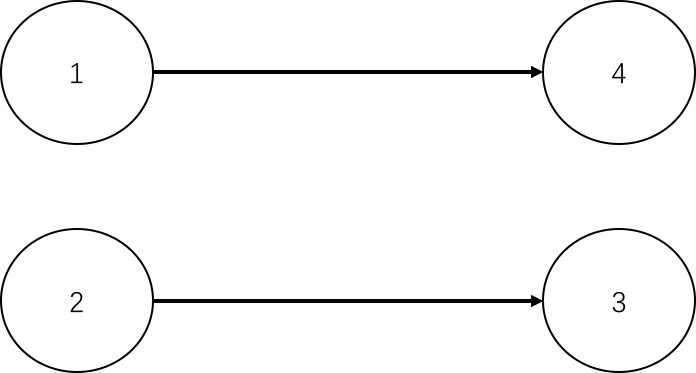
\includegraphics[width=0.4\textwidth]{interference}
  \caption{相邻链路干扰实验图示}
  \label{fig:interference}
\end{figure}

首先是相邻链路的信道竞争。图~\ref{fig:interference}给出了实验图示,节点1和节点3之间通信的同时
节点2和节点4通信,产生信道竞争,导致每条链路的实际有效带宽下降。
实验结果如下表~\ref{tab:interference}所示。

\begin{table}[htbp]
  \centering
  \caption{相邻链路干扰实验结果}
  \label{tab:interference}
  \begin{tabular}{p{2cm}p{2cm}p{2cm}p{2cm}p{2cm}p{2cm}}
  \hline
  发送功率 & 信道(L1-L2) & L1实际带宽(Mbps) & L2实际带宽(Mbps) & L1并发实际带宽(Mbps) & L2并发实际带宽(Mbps) \\
  \hline
  27 &  149-153 & 54.2 & 54 & 29.1 & 27.2 \\
  8 &  149-153 & 54.1 & 54.2 & 27.8 & 29.1 \\
  6 &  149-153 & 52.5 & 54.7 & 27.5 & 30 \\
  5 &  149-153 & 54.3 & 54.2 & 29.4 & 28.4 \\
  2 &  149-153 & 43.9 & 46.1 & 30.5 & 32.1 \\
  \hline
  \end{tabular}
\end{table}

可以明显看出当两条相邻链路同时发送数据时,各自的吞吐量降为原先的一半左右,当相邻的并发链路数量过多时
即可能导致每条链路的实际吞吐不足以支持视频流传输。

\subsection{隐终端}
隐终端指当网络中存在多个终端时,某终端只能在信道竞争时获知相邻终端的存在,而无法感知其他
更远处终端的存在,处于远处的未被感知的终端即称为隐终端。当某终端侦听信道判断当前信道空闲时,就会发送
数据,但可能与此同时远处的隐终端也认为信道空闲并发送数据,假设此时两份数据的接收者处于两者的物理位置
的中间,则两份数据同时到达将造成混乱,无法分辨,从而无法应答。导致两边的终端不得不反复的重传,甚至发生
数据包丢失。以下实验就是探究隐终端在Mesh网络中的影响。

首先进行单跳实验,网络拓扑如图~\ref{fig:hiddenterminal-1}。客户端连接N1节点,服务端连接
N5节点,图中共计5个节点组成一个稳定的无线Mesh网络。

在客户端和服务端之间,通过Mesh网络进行100次测试。每次测试运行20秒,客户端上的发送进程分别
以1至100间隔1Mbps的发送带宽向服务端发送UDP数据包。每次测量结束,服务端上的服务进程会统计
客户端此次通信数据的有效带宽、时延抖动等数据并告知客户端进程。所有测量结果在客户端汇总整理。

然后进行隐终端存在的实验,网络拓扑如图~\ref{fig:hiddenterminal-2}。客户端机器通过交换机与
Mesh网络中的N1节点和N5节点连接,服务端机器与Mesh网络中的N3节点相连,在该网络中,N1节点和
N5节点互相不在覆盖范围内,不知道对方的存在。
在客户端和服务端之间,客户端
虚拟两个进程,利用Iperf工具并控制N1节点和N5节点并发向N3节点发送数据,调节发射功率从500次
依次增大到1700,每次通过Mesh网络进行100次测试。每次测试进行20秒,客户端上的两个进程分别以
1到100间隔1Mbps的发送带宽向服务端发送UDP数据包。每次测量结束,服务端的进程统计客户端进程
此次通信数据的有效带宽等数据并告知客户端进程。所有测量结果在客户端汇总整理。
以上实验过程在N1节点和N5节点RTS/CTS打开与关闭的情况下分别进行依次。

\begin{figure}[H] % use float package if you want it here
  \centering
  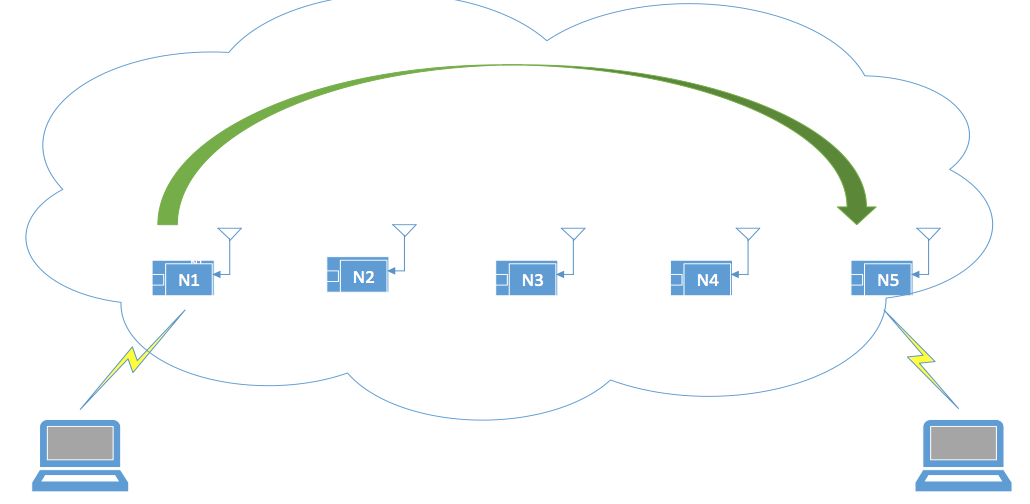
\includegraphics[width=0.8\textwidth]{hiddenterminal-onehop}
  \caption{单跳带宽测试}
  \label{fig:hiddenterminal-1}
\end{figure}
\begin{figure}[H] % use float package if you want it here
  \centering
  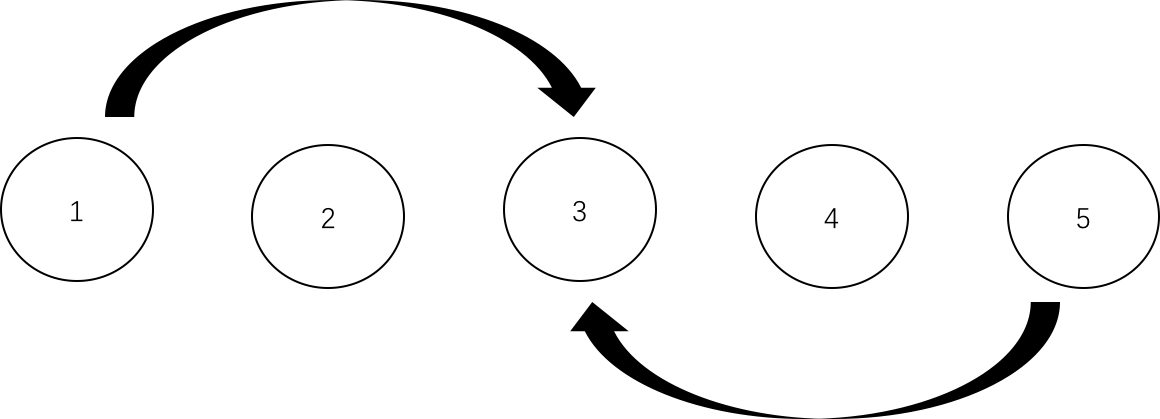
\includegraphics[width=0.8\textwidth]{hiddenterminal-hidden}
  \caption{隐终端带宽测试}
  \label{fig:hiddenterminal-2}
\end{figure}

单跳带宽测试实验结果如图~\ref{fig:hiddenterminal-3}所示,可以看到
在无干扰情况下,硬件平台支持的最大带宽接近100Mbps。

相较之下,隐终端存在的带宽测试实验结果如图~\ref{fig:hiddenterminal-4}所示,
该图示中同时呈现了RTS/CTS打开和关闭情况下实际有效带宽。可以明显看出RTS/CTS打开情况,实际有效
带宽提升在10Mbps至20Mbps。但考虑到RTS/CTS打开,因为需要发送RTS/CTS控制帧,所以会造成一定
程度上的额外资源开销。

进一步引入发送功率
作为因变量。之所以考虑发送功率,是因为发送功率和干扰范围密切相关,当发送功率升高时,
其干扰范围就会扩大,从而导致网络整体吞吐量下降。反之,发送功率过小,则会导致网络形成
更多的多跳路由,而每多一跳同样会带来额外的干扰。依次我们对发送功率同样进行了细致的实验
辅助建模,探索其和有效带宽的关系。

实验结果如图图~\ref{fig:hiddenterminal-5}所示,可以发现当发送带宽较小,即使较小的发送功率
也可以满足要求。但当发送带宽超过50Mbps后,发送功率就会成为限制有效带宽的一个重要因素,随着
发送功率进一步增大,有效带宽逐渐达到饱和。

综合发送带宽和发送功率绘制图~\ref{fig:hiddenterminal-6}。可以看到RTS/CTS打开的情况下,
有效带宽呈现出更好的状态。因此在实际项目系统的测试和部署中,如不特殊说明,将选择打开RTS/CTS
功能。

\begin{figure}[H] % use float package if you want it here
  \centering
  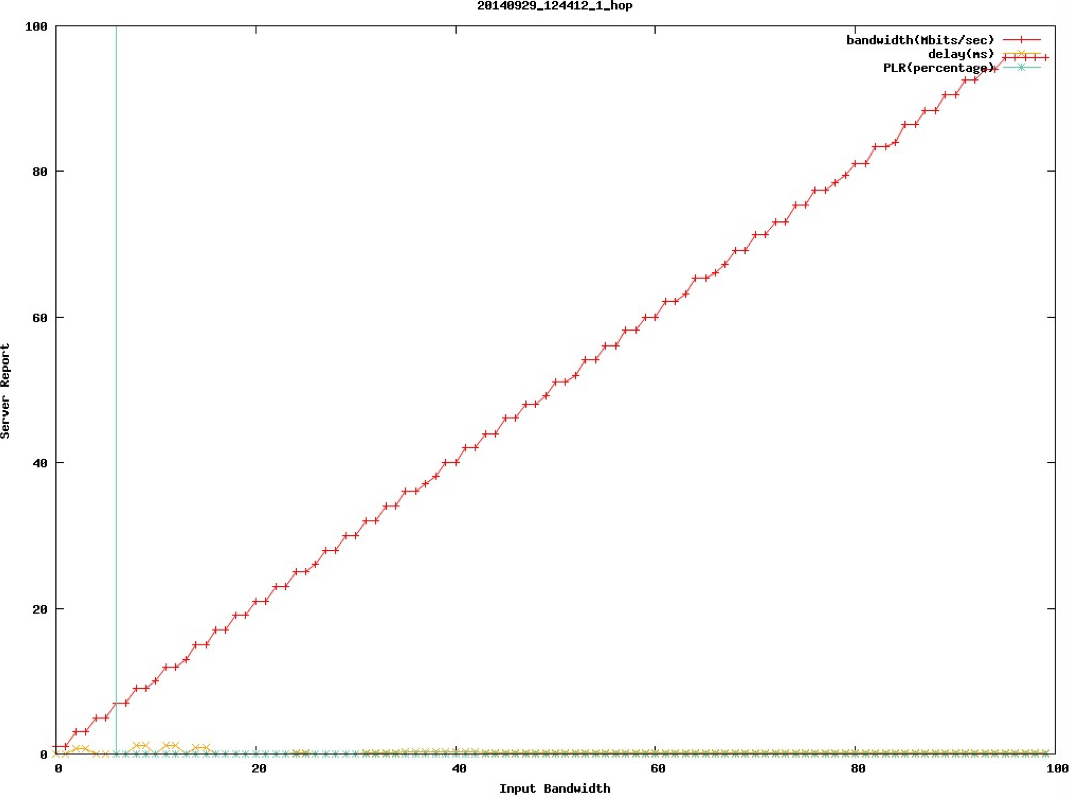
\includegraphics[width=0.8\textwidth]{hiddenterminal-onehop-result}
  \caption{单跳带宽测试实验结果}
  \label{fig:hiddenterminal-3}
\end{figure}
\begin{figure}[H] % use float package if you want it here
  \centering
  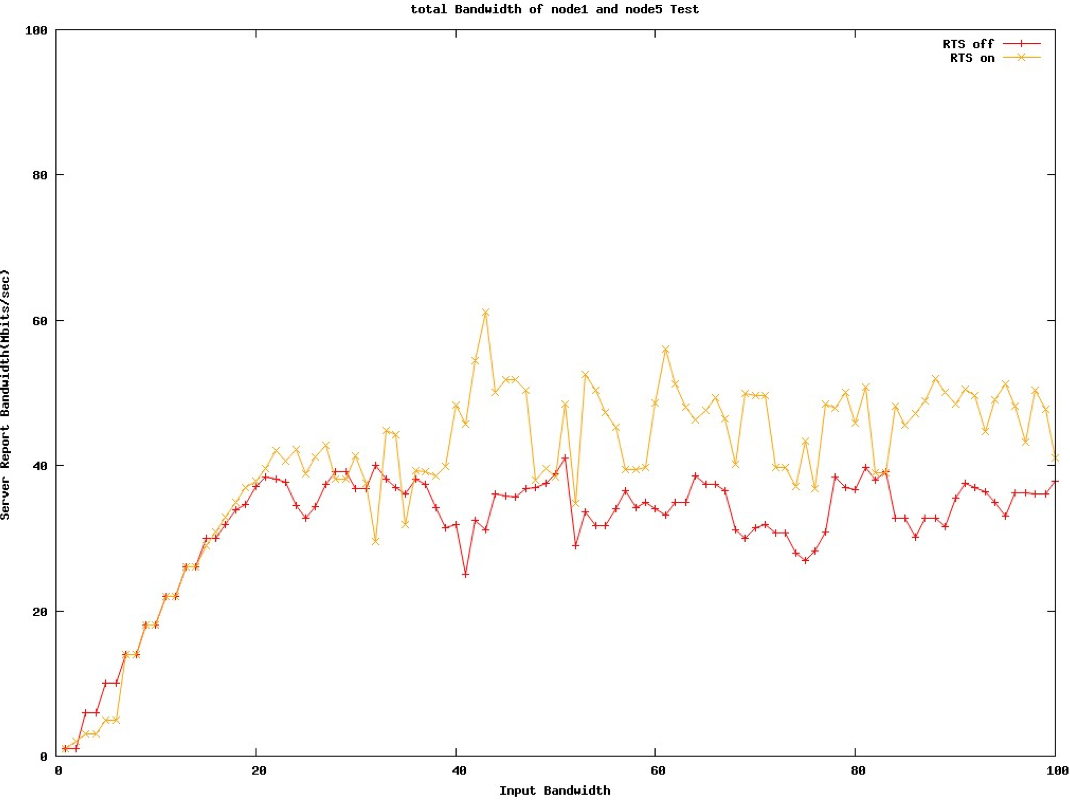
\includegraphics[width=0.8\textwidth]{hiddenterminal-rts-comp}
  \caption{隐终端带宽测试实验结果(rts打开vsrts关闭)}
  \label{fig:hiddenterminal-4}
\end{figure}
\begin{figure}[H] % use float package if you want it here
  \centering
  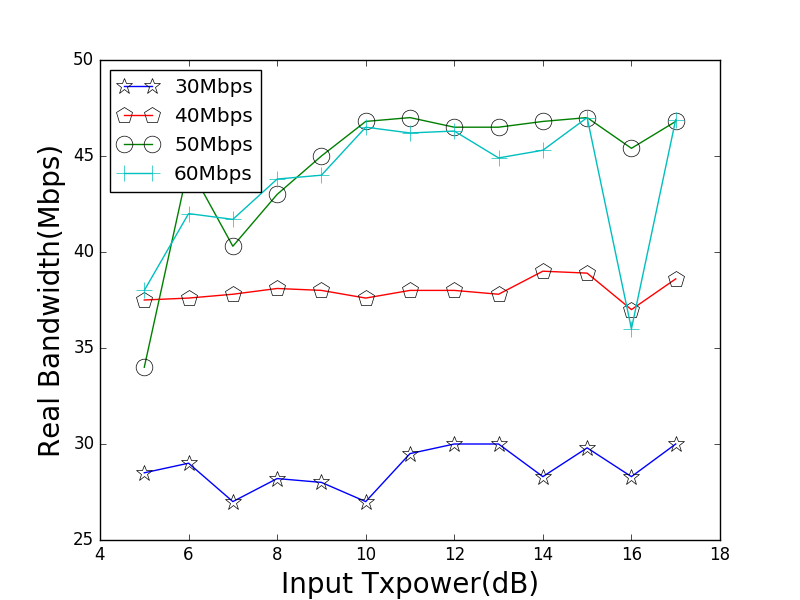
\includegraphics[width=0.8\textwidth]{hiddenterminal-txpower}
  \caption{发送功率对带宽影响}
  \label{fig:hiddenterminal-5}
\end{figure}
\begin{figure}[H] % use float package if you want it here
  \centering
  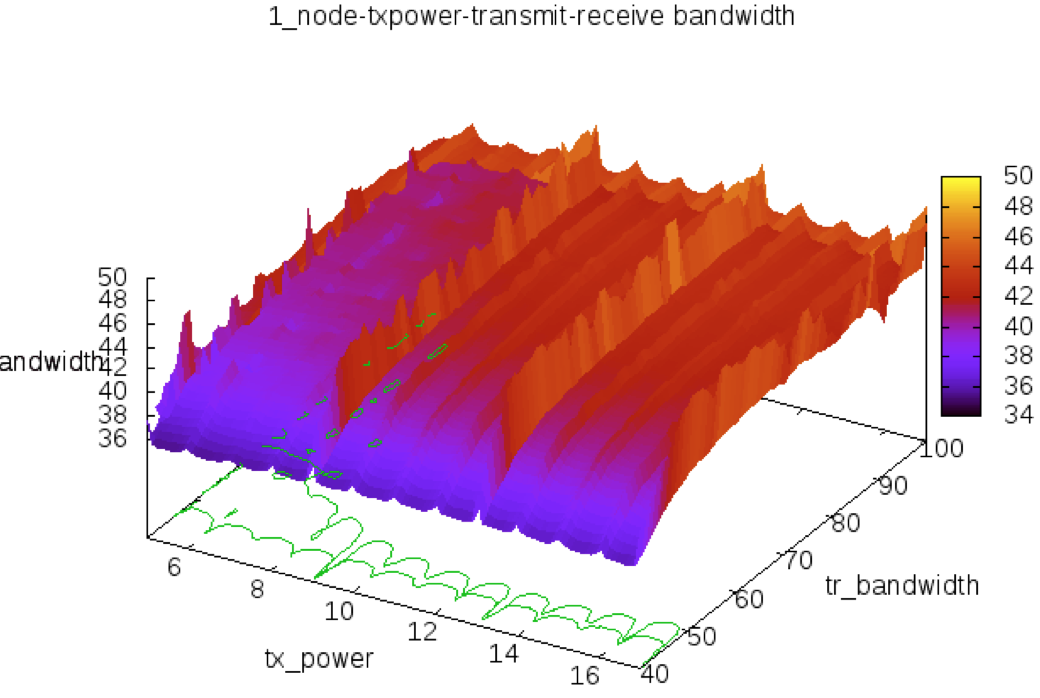
\includegraphics[width=0.8\textwidth]{hiddenterminal-rts-comp-3d}
  \caption{隐终端带宽测试实验结果(增加发送功率作为因变量)}
  \label{fig:hiddenterminal-6}
\end{figure}

由上述实验可以看出相邻链路干扰和隐终端的存在会给Mesh网络的实际有效带宽带来很大的干扰。
因此在进行总体网络规划的时候,选择进行子网划分,子网内部工作在同一信道,子网之间
采用正交信道,避免相互干扰。

5GHz在高频段有10个可用信道(根据所在国家和地区有差异)。设置20Mbps的信道宽度,则可以划分为
5个互相正交的独立信道。根据四色定理,平面空间中的区块可以用四种颜色着色,相邻区块不会出现
重色。据此,我们将整个网络划分为多个相邻的子网。子网内部独立自组织形成Mesh网络,每个子网
选择一个节点作为簇首节点,簇首节点作为该子网联通外部的网络的网关。上层簇首节点因为数量
可控,我们通过桥接形式接入远距离定向无线传输设备。这样最终的网络架构将是一种两层结构。
该结构既保留了Mesh网络的独特优势,又进一步通过分层分信道划分子网,到达隔离干扰域,优化
整体网络吞吐量的目的。

划分子网的另一个好处是,在我们的系统目标场景中,油田是一个重要的应用场景,而在野外的油田
分布十分分散,一套Mesh网络形成大范围覆盖效果并不理想,并且会需要大量的中继节点,
造成严重的资源浪费。为此我们可以在每一个油田或相邻的几个油田部署独立的一套
Mesh子网,完成对该油田区域的覆盖,可以提供充足的带宽用于监控、生产数据的传输。最终通过
簇首桥接远距离定向无线设备完成数据汇总至油田的控制中心。如[图]所示。

基于以上实验论证,我们搭建了较大型的室内实验平台,使用3.1节中介绍的硬件平台配置了101个Mesh
节点。将这101个节点划分为10个Mesh子网,每个Mesh子网的簇首桥接一个远距离无线设备,无线设备
与sink直接通信。实验平台如图~\ref{fig:subnet}所示。因为原硬件平台天线信号覆盖范围最大可达
3~5km,显然会造成整个实验床的全覆盖,形成严重的节点之间的干扰,实验验证在这种情况下视频
完全无法传输。于是我们给天线加装衰减器,通过调节衰减器的衰减性能将天线信号覆盖范围控制在
三米左右。这样可以基本保证划分的子网做到一定的区分。

\begin{figure}[h]
  \centering
  \subcaptionbox{}
      {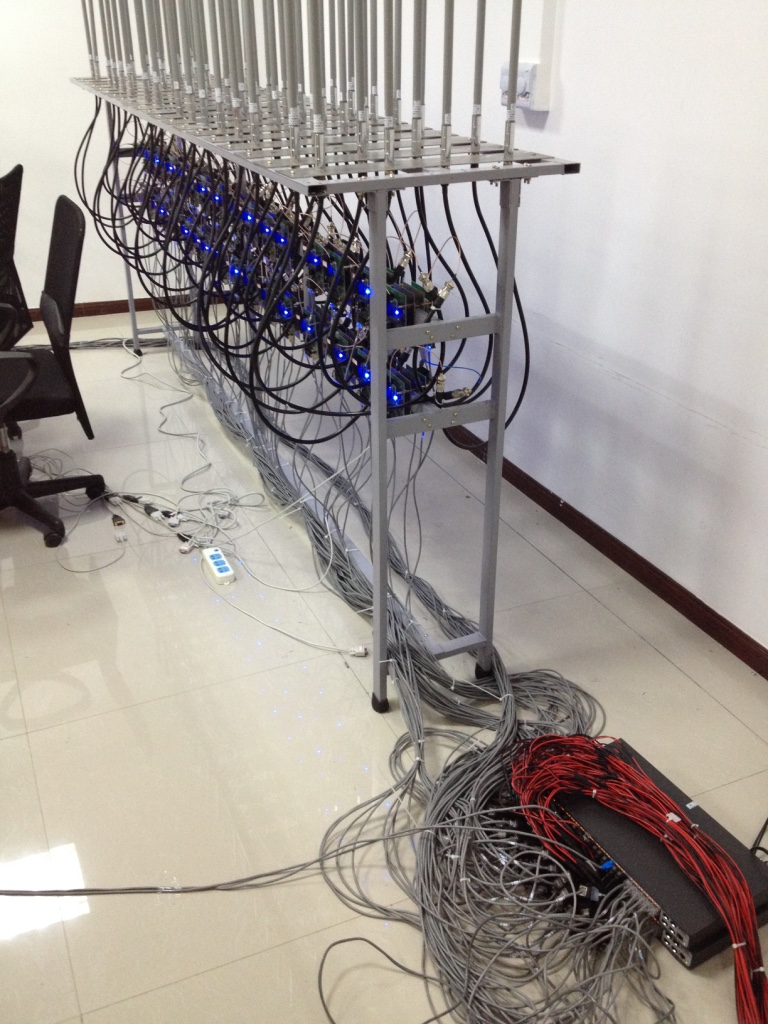
\includegraphics[height=5cm]{Subnet-3}}
  \hspace{1em}
  \subcaptionbox{}
    {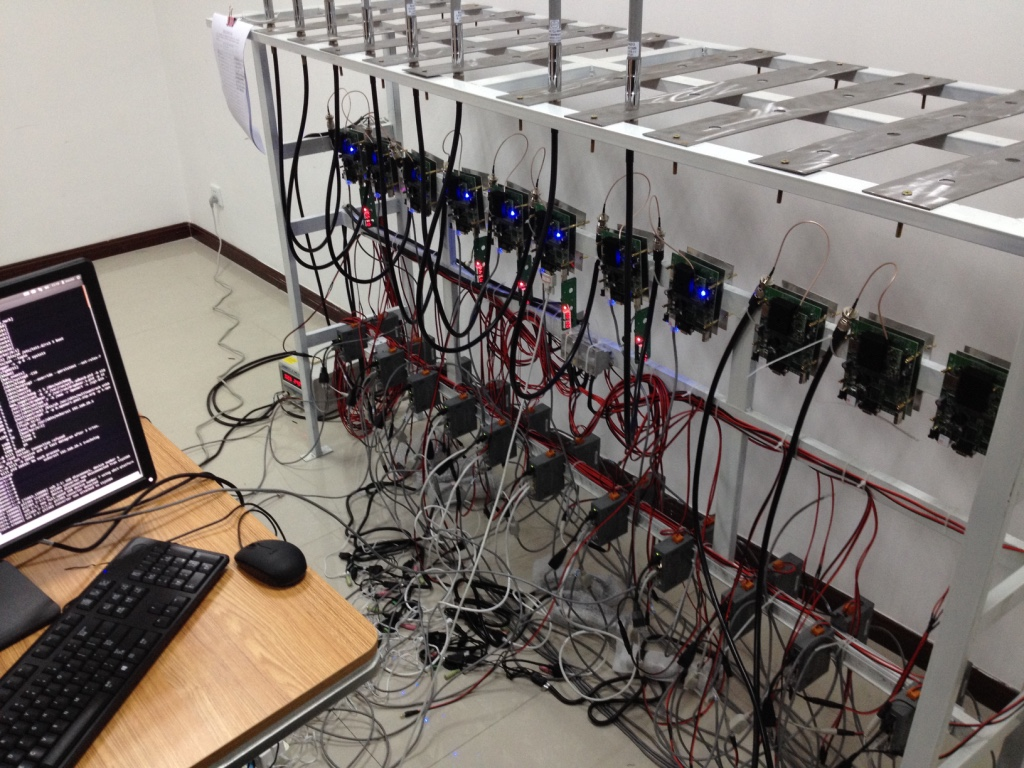
\includegraphics[height=4cm]{Subnet-1}}
  \hspace{1em}
  \subcaptionbox{}
    {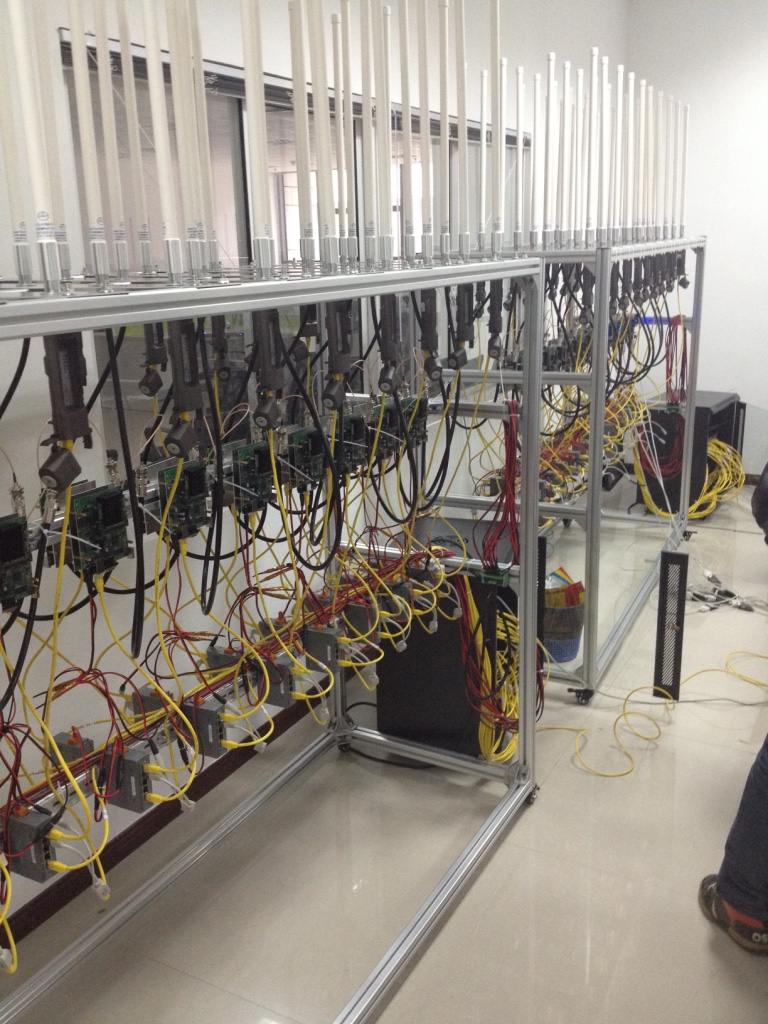
\includegraphics[height=5cm]{Subnet-2}}
  \caption{子网划分实验床}
  \label{fig:subnet}
\end{figure}

\begin{figure}[H] % use float package if you want it here
  \centering
  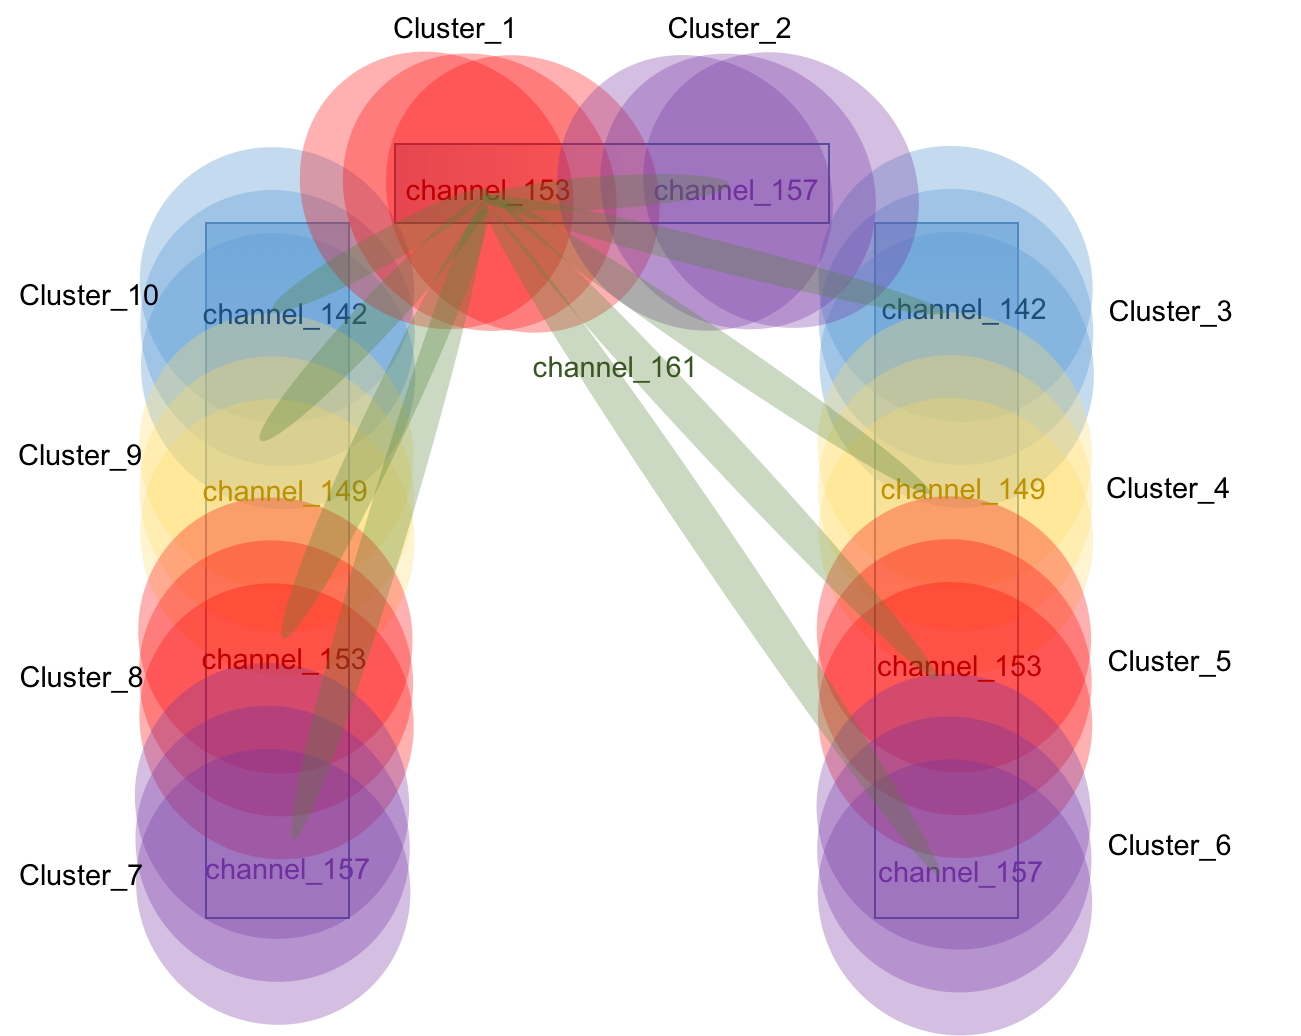
\includegraphics[width=0.6\textwidth]{Subnet-interference}
  \caption{子网划分后的干扰示意图}
  \label{fig:subnet_interference}
\end{figure}
实验床的节点物理位置分布成如图~\ref{fig:subnet_interference}所示,图中每种颜色代表一个独立的信道,
相互正交,相邻信道间隔知道为两个独立信道,因此不存在干扰。图中蓝、黄、红、紫分别代表5GHz频段
的142、149、153、157号信道,这四个信道用于分配给子网,根据四色定理,存在这样的方案使得
任意相邻信道之间不存在干扰。因为不同子网间节点在不信道,互相之间不可见,因此组网协议在不同
子网间也是不可组网的,这样就实现了子网的隔离,而子网内部可以自由组网。

这样的子网是
相互独立的,而我们最终需要的是一个整体的网路,因此我们使用两层架构,在子网之上,每个子网的簇首
节点桥接一个上层节点,该节点采用定向发送方式,因此虽然需要更高的传输功率但干扰范围可控,
且独立占据一个与所有子网都不相互干扰的信道。

完成配置部署后我们进行了实验验证,该方案带来的性能提升十分巨大,如表~\ref{tab:subnet_comp}所示。
实验比较了不同的信道划分方案,主要分两类,一种是所有节点均采用同一信道,全干扰状态下进行视频
传输实验,另一种是上述子网划分方案。在第一种单一信道实验中,用三种不同且相互正交的信道分别
进行,以排除环境种可能的信号干扰。在每个子网中接入3路视频,一共30路视频,每一路视频占用传输
带宽设置为2Mbps。实验结果以实际视频的传输质量为参照。

从表~\ref{tab:subnet_comp}中显而易见,子网划分方案带来的性能提升是显著的,单一信道在这样的
全干扰状态下几乎无法正常工作。
\begin{table}[htbp]
  \centering
  \caption{子网划分性能提升对比}
  \label{tab:subnet_comp}
  \begin{tabular}{|c|c|c|}
  \hline
  信道方案 & 实际效果 \\
  \hline
  单一信道方案(142信道) & 簇1内三路视频可见,簇2、簇3各一路视频可见 \\
  \hline
  单一信道方案(149信道) & 仅簇1内一路视频可见 \\
  \hline
  单一信道方案(153信道) & 仅簇1内一路视频可见,其他簇偶尔出现断断续续的视频 \\
  \hline
  子网划分方案 & 所有视频均可见,偶尔会出现卡顿现象 \\
  \hline
  \end{tabular}
\end{table}

\section{视频帧权重队列映射}
在过去的二十多年中,无线局域网中的视频流传输研究吸引了大量的研究人员的努力,其中很多的工作
都聚焦在QoS管理方面。比如,802.11e定义的EDCA,在mac层实现了不同的权重队列,每个队列对应
不同的发送优先级,上层过来的业务数据根据类型被映射到不同的权重队列中。视频和音频数据通常
具有更高的机会进入高优先级的发送队列。依次,相对于传统的802.11的信道竞争机制,EDCA的支持
下,视频音频数据将获得刚好的传输带宽,从而带来更好的用户体验。

另一方面,视频帧编码技术将视频编码为不同权重的帧,权重更高的帧对于视频的解析更重要,甚至
仅有高权重帧的情况下,也可以解码出流畅但不甚清晰的视频。由此,将视频帧帧解码为不同权重
的帧映射到不同的EDCA权重队列中,就可以实现在带宽资源过度匮乏的情况下,优先传输高权重
视频帧的目的。

目前,一些研究工作已经将这一想法引入了无线Mesh网络,但是并没有取得显著的效果。特别是在
网络规模扩大或者视频数据量增大的情况下,带宽很容易耗尽[Iptvhomenetworkingvia802.11 
wireless mesh networks: an implementation experience]。其他研究工作提出网络中的在线
视频数据削减[W 4: Real-time surveil- lance of people and their activities]。但是,计算机视觉技术会需要很大的资源开销,这对计算资源受限的mesh节点是一个
极大的挑战。另一方面,相关工作大多数都是通过仿真软件来完成,缺少实际系统的验证。

通过细致的实验分析,我们发现现阶段很多工作提出的映射机制和入队算法越来越复杂化,能够优化
的空间越发有限。一个可能的性能突破的方向是对数据进行更加细粒度的分析。例如对于视频数据帧,
不仅仅停留在编码帧的层面,而是深入观察相同的编码帧之间的差异,达到更好的映射效果。该想法
基于我们实验中的三点发现:
\begin{itemize}
\item[1.] 属于同一类型的编码帧在解码过程中的权重不同。典型的视频帧编码标准比如H.264和MEPG-4
将视频帧编码为三种不同类型的帧,分别是I帧、P帧和B帧。实验发现,属于统一个组的P帧权重依次递减,
B帧也呈现同样的规律。
\item[2.] 因为同一个编码帧可能在网络层或者更低层被分割为不同的数据包,这些数据包同样会呈现
不同的重要性。因此,在设计映射机制的时候,应该深入不同该层次的数据包,而不是停留在编码帧的
层面。
\item[3.] 映射机制应该具有足够的灵活性,使不同类型的编码帧都有机会使用高权重的发送队列,
最大限度的利用有限的带宽。
\end{itemize}

基于以上,本项目提出一种无线Mesh网络视频帧的mac层权重队列映射机制,全面的考虑了编码帧类型
、帧出现的位置、更细粒度的数据包形成最终的映射方案。该方案在高效的网络传输和有限的节点
计算资源之间做到很好的平衡。

\subsection{视频帧分层编码}
视频数据一直是数据量最大的业务数据类型,再如今大数据火热的阶段,尤其被关注,在无线网络中
视频数据同样也给网络传输带来了极大的挑战。不同的视频编码技术应运而生,在这之中,H.264和
MPEG-4被业界广泛接收和使用。这种类型的编码方式在性能和编码复杂度上都能够很好的满足大多数的
应用场景。

分成编码技术将视频编码为三种不同类型的帧:I帧、P帧、B帧。每一种帧在视频解码时都扮演不同的
角色。
\begin{itemize}
\item I帧(帧间编码):该帧数量最少,包含全部用来解码其自身的信息,这就以为这I帧的解码不需要
依赖其他I帧或者P帧、B帧。I帧通常压缩为一个静态图像,体态也较P帧、B帧更大。
\item P帧(前向预测帧):该帧包含它之前最近的I帧和P帧之间的差异,因此需要依赖之前的I帧和P帧来
解码。
\item B帧(双向预测帧):该帧压缩尺度最大,需要依赖其之前和之后的I帧和P帧来解码。
\end{itemize}

\begin{figure}[H] % use float package if you want it here
  \centering
  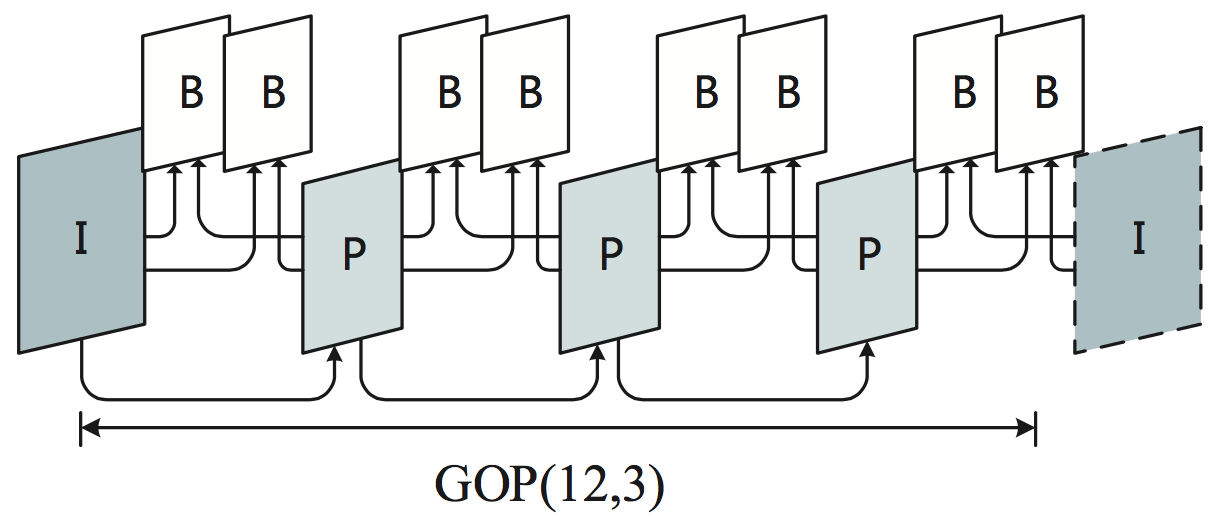
\includegraphics[width=0.6\textwidth]{GOP}
  \caption{GOP结构示例,GOP(12,3)}
  \label{fig:gop}
\end{figure}
根据H.264和MPEG-4编码,一小段视频会被解析编码为一组重新组织过的帧,这一组帧称为GOP。每个
GOP总是由一个I帧开始,之后跟随一段连续的P帧和B帧。GOP的结构可以表示为两个参数G(N,M),其中
N表示GOP中包含的所有帧的数量(两个连续I帧之间的距离),M表示I帧和其后第一个P帧之间(
或者两个连续P帧之间)的距离。图~\ref{fig:gop}为G(12,3)的结构示例,分解后即为:‘IBBPBBPBBPBB’。

如图~\ref{fig:gop}所示,GOP内部的不同帧之间紧密相连,不同的GOP之间相互独立。实质上,I帧不
依赖于任何其他帧,可以单独解码,P帧依赖于其之前的I帧或者P帧,B帧依赖于其前后的I帧或者P帧。
也就是说,如果在传输过程中,丢失了I帧则整个GOP都无法解析。类似的如果一个P帧丢失,则其后
的P帧和B帧均无法解码。而B帧丢失仅影响其自身,其他数据帧不会收到任何影响。由此我们可以总结
三种类型帧的重要性,显然I帧>P帧>B帧。

综上,处于QoS保障的考虑,当带宽紧缺时,需要保证重要性更高的帧优先传输。

\subsection{802.11e增强分布式协调访问(EDCA)}
传统的IEEE802.11标准分布式信道接入协调功能(DCA)最为基础的信道接入方式,该方式基于CSMA/CA,
不提供QoS保障。为了支持区分的服务,802.11e引入了一种混合协调功能(HCF),其中包含两种并行
机制:混合控制信道访问(HCCA)和增强分布式协调访问(EDCA)。本项目中基于EDCA功能展开。

EDCA通过引入四个不同的接入类型(AC)来提供QoS保障。传统的802.11信道接入方式维护一个发送队列,所有
业务数据平等的进行信道竞争,不同于此,每个AC的数据维护各自的发送队列,通过竞争窗口控制
每个队列竞争获得信道的概率不同。如图~\ref{fig:acofedca}所示,四个队列按权重从低到高依次是:
AC\_BK(背景数据),AC\_BE(尽最大努力传送),AC\_VI(视频),AC\_VO(声音),依次编号为AC(0),AC(1),
AC(2),AC(3)。不同的权重通过设置不同的信道竞争参数实现,包括竞争窗口界限、仲裁帧间隔、
发送机会限制。

默认情况下,QoS支持在EDCA中的实现是通过将实时数据包括音频视频映射到AC(2)和AC(3)中,其他的
数据则映射到AC(0)和AC(1)。EDCA机制不考虑视频帧的不同类型之间重要性的区别,将所有的编码都
映射到AC(2)中。然而,在视频监控的场景中,除了少量的控制数据,几乎所有的数据都是视频数据,
这些数据都被映射到同一队列,很容易造成该队列的饱和,进一步造成丢包,影响传输质量。因此,在
无线Mesh网络中,尤其在视频流作为主要传输数据的场景中,应该充分挖掘视频帧编码之间的差异,
利用EDCA四个队列的功能来实现更好的用户观看体验。之前已经有一些工作做过这方面的尝试,图
~\ref{fig:originmapping}给出了静态映射和动态映射的对比。静态映射,比如[Ieee 802.11 e wireless lan for quality of service]
,仅仅将不同重要性的帧固定的放入固定的队列,这样会造成优先队列资源的浪费。动态映射,比如
[Adaptive scheduling for wireless video transmission in high-speed net- works],进一步考虑
网络地动态状况和队列地占用情况,动态地进行队列映射,提高了网络地利用度。

\begin{figure}[H] % use float package if you want it here
  \centering
  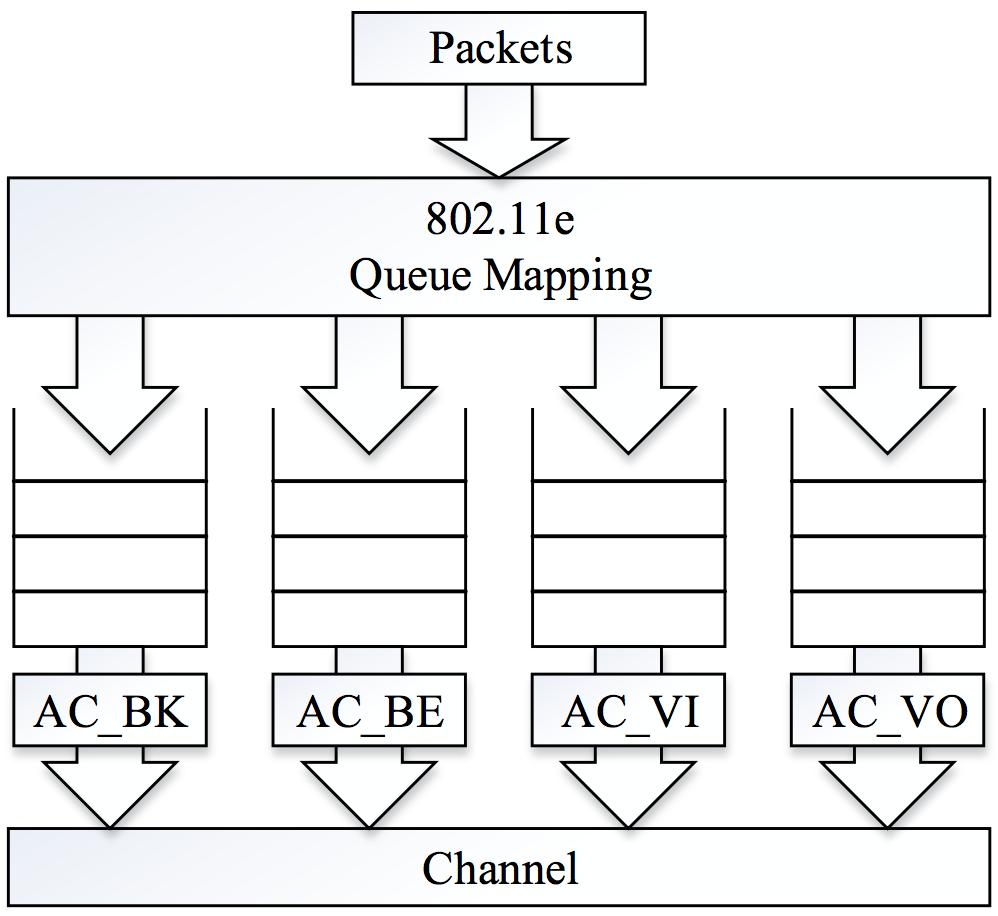
\includegraphics[width=0.6\textwidth]{ACofEDCA}
  \caption{EDCA的四个AC队列}
  \label{fig:acofedca}
\end{figure}
\begin{figure}[H] % use float package if you want it here
  \centering
  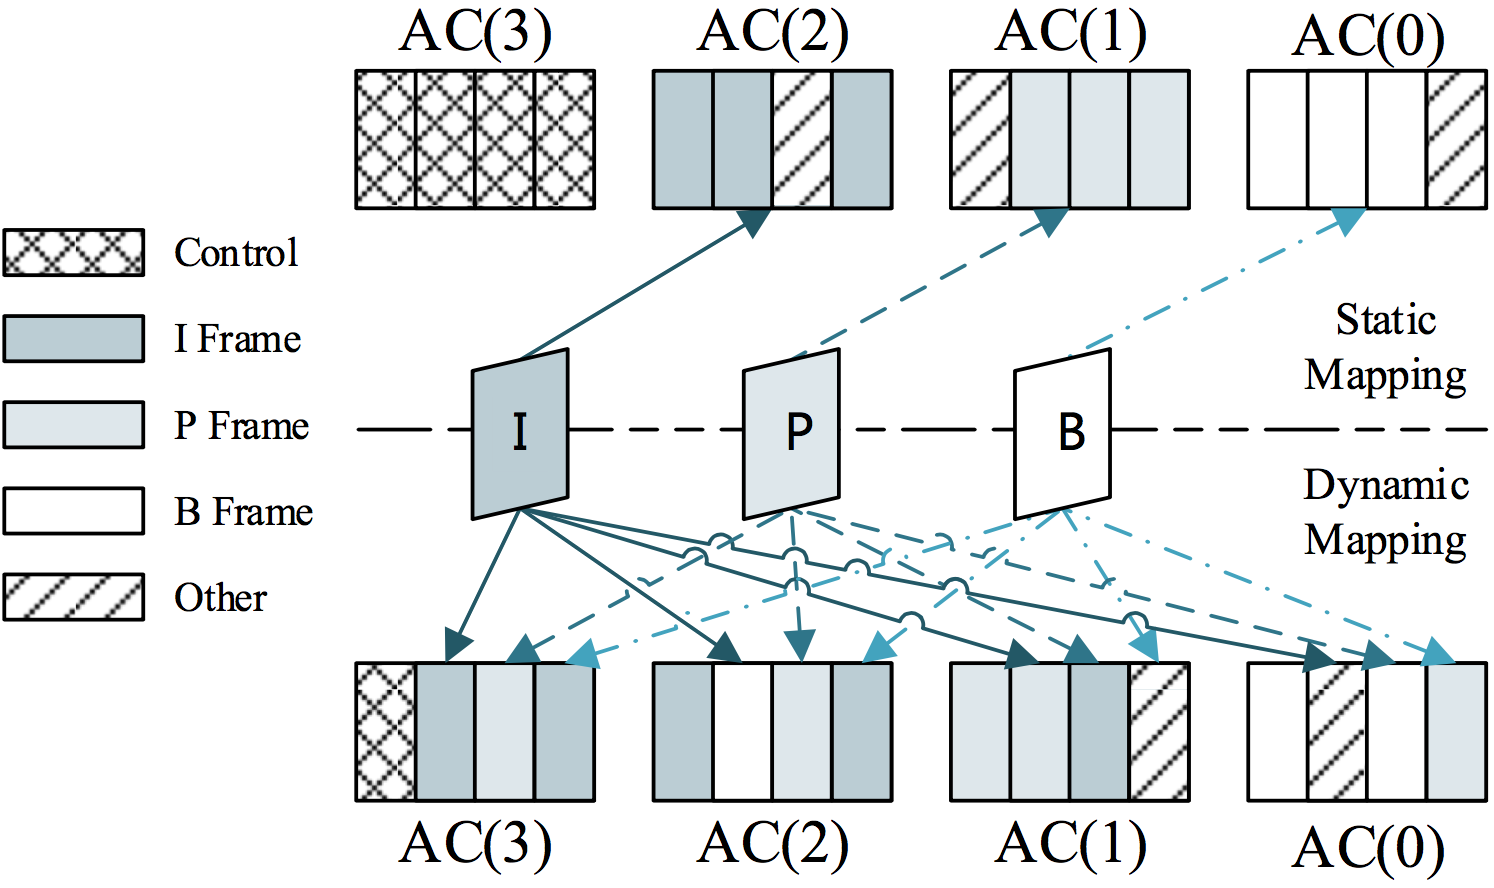
\includegraphics[width=0.6\textwidth]{mapping}
  \caption{静态映射和动态映射机制示例}
  \label{fig:originmapping}
\end{figure}

\subsection{视频帧映射机制}
基于GOP编码结构和EDCA机制,结合细粒度地分析视频数据包,我们提出了一种跨层映射方案,实验显示该
所提方案相对于朴素地基于EDCA传输方案,优化效果>50\%。

在视频监控系统中,视频数据占所传输带宽的绝大部分。在衡量视频传输质量的时候,除了传统网络
度量参数如丢包率等,更重要的是视频观看体验,目前普遍使用的衡量指标是峰值信噪比(PSNR)和结构
相似性指标(SSIM)。视频传输的流畅、实时、清晰是视频监控系统的首要目标。

受通用视频编码技术中的分层编码的影响,可以认为不同类型的帧对视频的传输质量贡献不同。这是由
分层编码中GOP内部不同帧之间的依赖关系决定的。如前所述,I帧独立于其他帧,可独立解码
其压缩率也最低;P帧依赖于其之前的I帧或者P帧,压缩率次之;B帧压缩率最高,但需要依赖其前后的
I帧或者P帧来解码。不难发现,I帧丢失则该GOP内全部的帧都无法解码;P帧丢失则其后的所有帧无法
解码,B帧丢失则仅其自身无法解码,不影响其他帧。

\begin{figure}[H] % use float package if you want it here
  \centering
  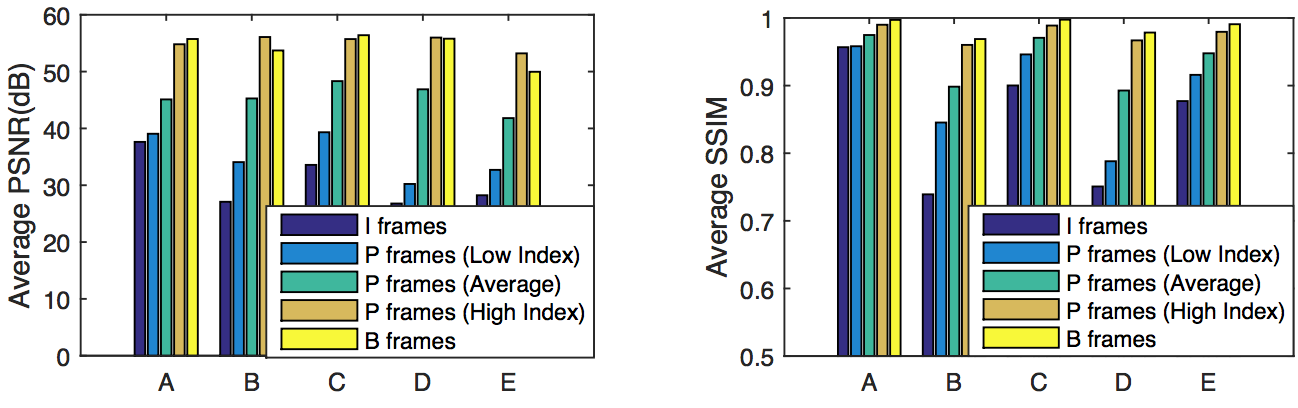
\includegraphics[width=0.8\textwidth]{IPB-comp}
  \caption{I帧、P帧、B帧丢失对视频质量的影响比较}
  \label{fig:ipb-comp}
\end{figure}
\begin{figure}[H] % use float package if you want it here
  \centering
  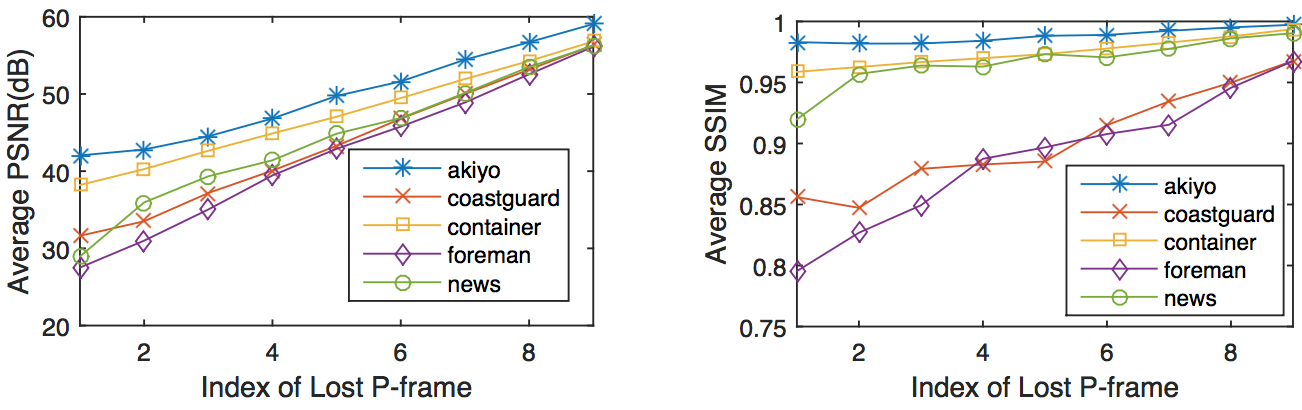
\includegraphics[width=0.8\textwidth]{Position-comp}
  \caption{不同位置的P帧丢失对视频质量的影响比较}
  \label{fig:position-comp}
\end{figure}

图~\ref{fig:ipb-comp}和图~\ref{fig:position-comp}
给出了I帧、P帧、B帧以及同一个GOP中不同位置的P帧丢失对视频质量的影响。可以看出,和我们预测
的相同,在相同的数量上上,I帧对视频质量的贡献明显大于P帧,P帧中出现在靠前位置的P帧影响力
又要大于之后的P帧,而B帧对视频质量的影响最小。

之前的关于映射机制的工作,仅仅按照编码帧的类型进行映射,而没有考虑不同位置帧的重要性不同。
我们将这一点引入映射机制,综合考虑帧的\emph{类型}和\emph{位置}。下面详细介绍该映射机制的
细节原理和实现。其中核心分为两部分,帧权重计算和帧映射。

\begin{table}[htbp]
  \centering
  \caption{本章符号检索}
  \label{tab:notations}
  \begin{tabular}{p{3cm}p{8cm}}
  \hline
  符号 & 信道(L1-L2) \\
  \hline
  N, M &  GOP参数 \\
  $\omega$ &  数据包权重值 \\
  $f_{0}$ & 受当前帧影响的帧数量 \\
  $f_{1}$ & 影响当前帧的帧数量 \\
  $\alpha$, a, b & 权重值计算公式参数 \\
  $b_{0}$ & 权重值基线 \\
  h & 帧分解的第一个数据包的额外权重 \\
  p & P帧在GOP中的位置索引 \\
  \emph{threshold(i)} & AC(\emph(i))的最大队列缓存 \\
  \emph{qlen(i)} & AC(\emph(i))当前使用长度 \\
  \hline
  \end{tabular}
\end{table}

\renewcommand{\thesubsubsection}{\Alph{subsubsection}.}
\subsubsection{权重计算}
对于I帧,因为其相对于P帧和B帧数量极少,且对于解码GOP起到至关重要的作用,所以在权重上赋最
大值1,即为$\omega =1$;对于P帧和B帧,它们的重要性和它们之前的需要依赖的帧以及它们后续的
依赖于它们的帧有关。这里我们定义受当前帧影响的帧数量为$f_{0}$,对当前帧有影响的帧数量
为$f_{1}$。进一步的定义当前帧的权重计算公式为:
$$ \omega = g(f_{0}\alpha^{f_{1}}) $$
在这里,$\alpha \in (0,1)$是一个权重常量,用来平衡$f_{0}$和$f_{1}$,$f_{0}\geq1$(所有的P
帧和B帧至少被I帧影响),$f_{1}\geq1$(每一个帧至少影响它本身),g(x)是一个单调递增函数。
这就意味着,越多的帧依赖于当前帧,或依赖于当前帧的帧越少,则当前真的权重就越高。更直观
的讲,就是在一个GOP中出现越早的帧相对于晚出现的帧权重更高。

为了降低Mesh节点的计算开销,g(x)定义为:
$$ g(x) = a(\log (x) + b) + b_{0} $$
带入$\omega$表达式则有P帧和B帧数据包的权重值计算公式:
$$ \omega = a(\log f_{0} + f_{1}\log \alpha + b) + b_{0} $$

上式中,$b_{0}$是作为权重值的基线,确保B帧能够有机会进入优先级较高的队列。a、b和$b_{0}$
用来限制$\omega$在[$b_{0}$,1]的范围内。可推出a,b值如下:
$$ a = \frac{1-b_{0}}{\log(N) - \log(\alpha^{N/M})} $$
$$ b = -\log(\alpha^{N/M}) $$

上式中,$\log(N)$和$\log(\alpha^(N/M))$分别为$\log(f_{0}\alpha^f_{1})$的最大值和最小值。
对于一个GOP中的第\emph{p}(\emph{p}>0)个P帧,$f_{0}=N-1-M*p$, $f_{1}=p$。对于任意子第
\emph{p}个P帧后的B帧,有$f_{0}=1, f_{1}=2$。

目前为止,我们定义了普通的视频帧数据包的权重计算方法,该方法充分利用的GOP结构中不同\emph{类型}
帧不同的重要性。下面我么考虑利用同\emph{类型}不同\emph{位置}帧重要性不同的性质,其中关键
的是一个视频帧被底层协议拆分为一个个的数据包时,最重要的是第一个数据包,其中包含了编码重要
的信息。我们选择添加一个额外的值\emph{h}来提升第一个数据包的权重。如果出现$\omega+h>1$,就设置
$\omega=0.99$。之所以这里不设$\omega$为1是考虑到防止P帧或者B帧抢占I帧的优先权,在保证I帧
绝对优先权的基础上最大限度提升P帧或者B帧较重要的数据包的传输几率。

\subsubsection{帧映射}
所谓帧映射就是将属于不同类型帧的数据包映射到不同的EDCA的AC中,区分他们在发送时的优先权。
根据上一节涉及的权重计算方法,可以计算出每一个视频帧对应的权重值,帧映射即可以根据该权重值
完成。映射的直接原则是充分使用高权重队列以降低传输延迟和丢包率。当网络质量良好,传输数据量
较小时,甚至可以将B帧映射到AC(0)中,所有帧都可以以最低延迟,最高的优先权完成传输。相反,
当网络质量较差,网络传输数据量过大,造撑拥堵时,映射机制优先将I帧映射到最高优先权队列,保证
I帧的传输质量。

当一个数据包到达时,映射机制将顺序从最高优先权队列AC(3)开始依次检测。如果发现当前AC有足够的
缓冲区余量,且满足映射标准,即将数据包插入该AC中。判定的标准为,给定一个数据包的权重假设
为$\omega$,如果$\omega*threshold(i)>qlen(i)$,就将数据包插入队列AC(\emph{i});否则,继续
检查优先权次之的队列。其中,$threshold(i)$和$qlen(i)$是AC(\emph{i})可以通过底层API读取的
最大队列长度和当前队列占用。如果一个数据包不能够插入AC(3),AC(2)和AC(1),那么就直接插入AC(0)
而不需要进行进一步的检查。映射算法尽可能设计的简单以减少Mesh节点的计算开销,因为在工业应用
中,Mesh节点能源和计算资源都比较稀缺。

上面的队列映射策略给予了更高权重的数据包更高的概率插入高优先级队列,同时阻止低权重的数据包
阻塞队列。

\subsubsection{映射系统实现}
队列映射如图~\ref{fig:workingflow}所示,跨层架构设计也在图~\ref{fig:crosslayer}中展示。
在结构设计上,因为BATMAN-adv协议主要工作在mac层,且EDCA的四个AC也在mac层实现,所以我们的
权重计算和映射模块均在mac层实现。尽管如此,我们需要在考虑来自引用层的数据,网络层的ToS字段,
以及物理层的队列大小及占用情况。实际系统中,每个视频帧的数据包,其权重均在产生该数据包的
第一个Mesh节点计算。当一个Mesh节点接到请求需要发送视频数据时,首先解构GOP为I帧、P帧和B帧,
然后将各个帧在网络层封装为较小的数据包,之后就根据每个数据包所属帧的类型、位置和数据包是否
为帧的头数据包等计算数据包的权重。之后数据包的权重值一值维护在数据包中,在网络传输的过程中
不会改变该权重值。在最近的实现中,我们将权重值存储在网络层包头的ToS字段中。

数据包传输到网络中间任一节点时,该节点队列映射也按如图~\ref{fig:workingflow}所示进行,
但不需要重新计算权重值,只需要从ToS字段中取的该权重值即可,之后就根据该权重值,将数据包
插入相应的AC中。

\begin{figure}[H] % use float package if you want it here
  \centering
  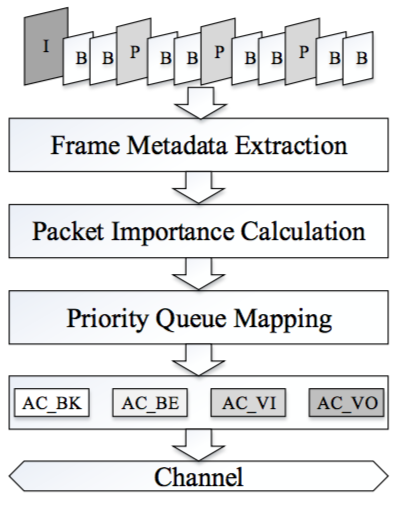
\includegraphics[width=0.4\textwidth]{WorkingFlow}
  \caption{映射机制流程}
  \label{fig:workingflow}
\end{figure}
\begin{figure}[H] % use float package if you want it here
  \centering
  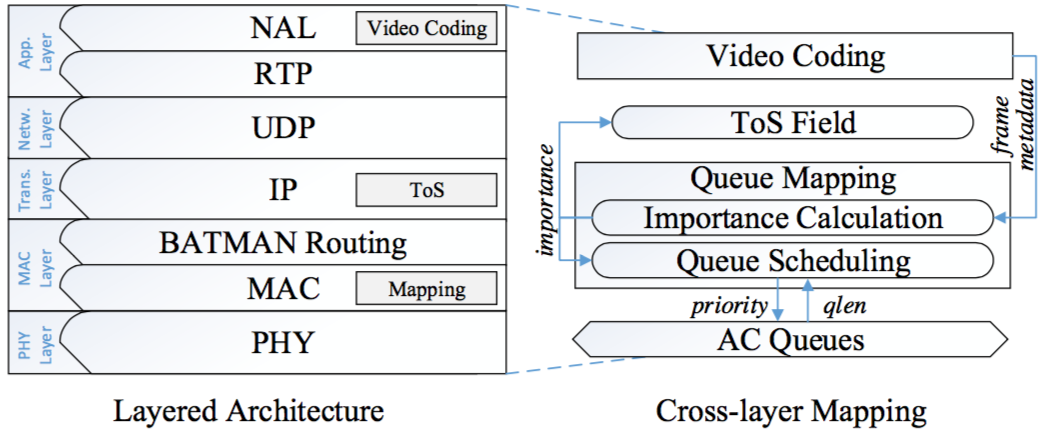
\includegraphics[width=0.8\textwidth]{Crosslayer}
  \caption{映射机制跨层设计}
  \label{fig:crosslayer}
\end{figure}

\subsection{实验验证}
\renewcommand{\thesubsubsection}{\Alph{subsubsection}.}
\subsubsection{实验方法}
在3.1节已经介绍了项目所采用的软件系统和硬件平台。更细致地,OpenWRT内置的\emph{mac80211}模块
控制数据包的收发。\emph{队列选择}是数据包发送过程中的一个子环节。





\section{移动场景下的QoS保障}
无线Mesh网络目前还处在一个高速发展的阶段,不管是学术界还是工业界目前都还在尝试不同的技术。
在物理层上,MIMO、多无线模块、软件无线电等技术都被尝试应用到Mesh网络中以获得更好的网络性能。
链路层上,QoS技术、时分复用技术等也被广泛他所应用。网络层上更是围绕组网协议这一核心模块集中
了大量的研究工作,在2.2节中已经列举了诸多目前正在使用的Mesh组网协议,它们在链路选择、组网方式
上或多或少都存在差异,而这些协议目前共同面对的一项挑战就是不能很好的应对移动场景下的漫游的
切换时延问题。

本节的工作就是聚焦在移动场景下如何保证客户端接入在不同的Mesh主干网络节点之间切换是做到无缝零
时延。这是一项极具挑战性的工作。












